\chapter{Analyse}

\authoredsection{Laura}{Lernprozess}
Dieser Abschnitt widmet sich einer eingehenden Analyse des Lernprozesses auf der Plattform. Der Fokus wird unter anderem auf verschiedene Ansätze und Theorien zum digitalen Lernen und zur Motivierung der Lernenden gesetzt.
Der Lernprozess spielt eine herausragende Rolle, da er direkte Auswirkungen auf den Wissenserwerb und die Motivation beim Lernen hat.

Zunächst werden die Anforderungskataloge beschrieben, die als Grundlage für die Lektionen dienen. Die einzelnen Elemente und die Struktur dieser Kataloge werden erläutert, um ein besseres Verständnis für den weiteren Verlauf der Arbeit zu schaffen. 
Anschließend werden die Struktur der Übungen sowie die verschiedenen Aufgabentypen vorgestellt, die auf der Lernplattform angeboten werden sollen.

\subsection{Anforderungskatalog}
Die Anforderungskataloge nehmen eine zentrale Rolle bei der Erstellung von Übungsaufgaben ein. Durch sie können Aufgaben gezielt auf funktionale Anforderungen und Produkte ausgerichtet werden, die einer Bewertung unterzogen werden sollen.
Zunächst wird der allgemeine Aufbau eines solchen Anforderungskatalogs vorgestellt. Im Rahmen dieser Projektarbeit wurden Beispielkataloge und Aufgaben von Professor Hoffmann bereitgestellt. Mithilfe eines Beispielkataloges lässt sich der Anforderungskatalog genauer erläutern.
Ein Ausschnitt eines solchen Beispielkatalogs ist in der folgenden Tabelle \ref{fig:Anforderungskatalog-Bsp} zu finden.

\begin{figure}[H]
    \centering
    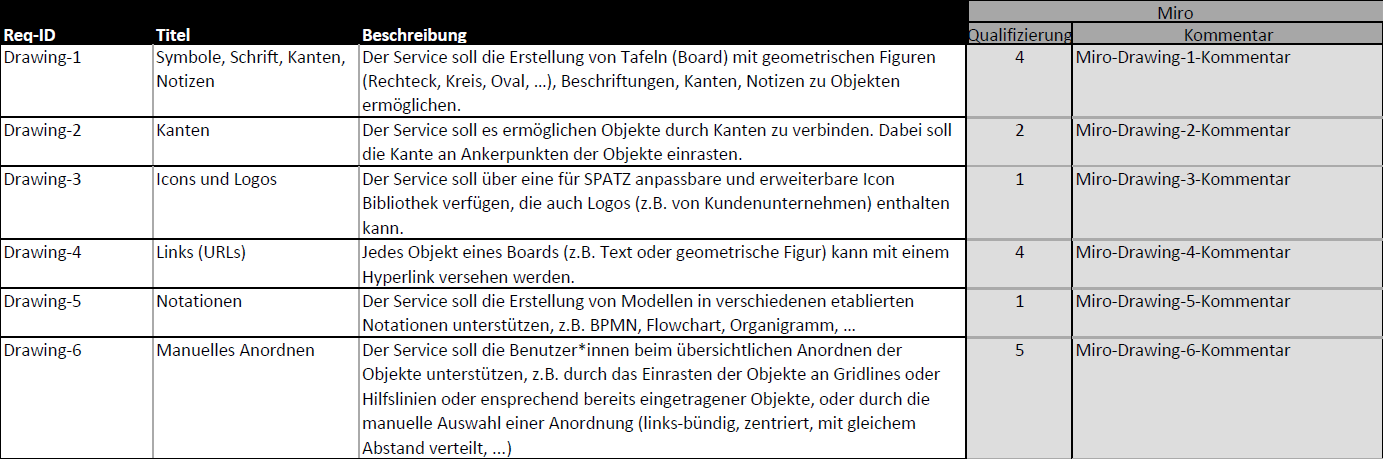
\includegraphics[width=1.0\textwidth]{assets/screenshots/kataloge/KatalogBspAusschnitt.png}
    \caption{Ausschnitt eines Anforderungskatalogs}
    \label{fig:Anforderungskatalog-Bsp}
\end{figure}

Diese Form von Anforderungskatalogen wurde bereits in Aufgaben für Wirtschaftsinformatiker an der FH verwendet. Dadurch dient sie als Grundlage für die Kataloge, die in die Lernplattform und die digitalen Übungen integriert werden.
Die Tabelle zeigt, dass jeder Katalog aus mehreren Anforderungen besteht, für die stets eine Identifikationsnummer (Req-ID), ein Titel und eine Beschreibung vorhanden sind. Dadurch wird klar definiert, was von einem Produkt erwartet wird.

Desweiteren ist in der Tabelle beispielhaft das Produkt \glqq Miro\grqq{}  eingetragen. Dieses Produkt besitzt weitere Spalten für die Qualifizierung und einen Kommentar. Die Qualifizierung beinhaltet einen Wert auf einer Skala von eins bis fünf. Der Wert beschreibt, in welchem Ausmaß das Produkt der Anforderung gerecht wird. Weiterhin kann der Kommentar z.B. als Begründung für die Qualifizierung dienen. Es ist zu beachten, dass es sich hierbei lediglich um einen Ausschnitt aus der Tabelle handelt, und es durchaus weitere Produkte und Anforderungen geben kann.

\subsubsection{Struktur} 
Nachdem die Inhalte der Anforderungskataloge genauer betrachtet wurden, wird nun analyisiert, welche Elemente in den Aufgaben unbedingt benötigt werden. Desweiteren wird eine geeignete Struktur der Kataloge für die Lernplattform ermittelt. 

Die Erstellung von Aufgaben mit Anforderungskatalogen sollte für die Lehrenden möglichst reibungslos gestaltet werden. Deshalb wird eine Struktur für die Kataloge festgelegt, die sich eng an den bereitgestellten Katalogen von Herr Professor Hoffmann orientiert.
Ein Ausschnitt eines solchen Anforderungskatalogs, der die Kriterien erfüllt, um hochgeladen zu werden, ist in Tabelle \ref{fig:Anforderungskatalog-Hochladen-Bsp} zu sehen. Dieser Katalog steht auf  der Lernplattform zum Runterladen zur Verfügung, so dass Lehrende diesen auch als Vorlage nutzen können.

\begin{figure}[H]
    \centering
    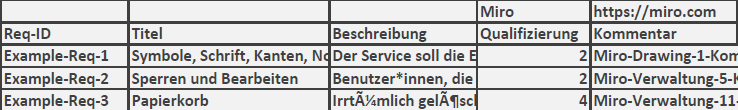
\includegraphics[width=1.0\textwidth]{assets/screenshots/kataloge/UnserKatalogBspAusschnitt.png}
    \caption{Ausschnitt eines Anforderungskatalogs im Format zum Hochladen}
    \label{fig:Anforderungskatalog-Hochladen-Bsp}
\end{figure}

Die grundlegenden Attribute des Katalogs von Professor Hoffmann wurden in die Tabelle übernommen. Darunter fallen die Anforderungen mit jeweils einer ID, einem Titel und einer Beschreibung. Die Produktattribute bleiben ebenfalls erhalten, allerdings wird zusätzlich eine URL ergänzt. Die Lernenden haben während der Übungen Zugriff auf diese URL. Dadurch erhalten sie einen Anhaltspunkt für die Evaluierung der Produkte. Auf diese Weise können die Lernenden die Produkte außerhalb der Lernplattform genauer betrachten, indem sie der URL folgen.

Um das Hochladen eines Kataloges zu erleichtern, wurden spezifische Kriterien entwickelt, die den Lehrenden als Hilfestellung dienen können. 
Die Datei mit dem Anforderungskatalog muss entweder eine CSV (Comma-separated values)\footcite[Vgl.][]{csv}{}{} oder eine XLSX Datei sein. Diese Formate eignen sich gut, da sich Tabellen häufig in diesen Formaten exportieren oder importieren lassen und die Weiterverarbeitung der Daten beim Hochladen ermöglicht wird. XLSX Dateien basieren auf dem XML Standard und werden daher von vielen Tabellensoftwaren unterstützt.\footcite[Vgl.][]{xlsx}{}{} Zudem erleichtert ihre Komprimierung die Weitergabe der Daten.\footcite[Vgl.][]{xlsx}{}{}

Für CSV-Dateien ist besonders auf eine korrekte Exportierung zu achten, da hier Spaltentrennungen nur durch Semikolons erkannt werden.

Die Kataloge sollten das gleiche Format wie im Beispielkatalog \ref{fig:Anforderungskatalog-Hochladen-Bsp} aufweisen, um ein fehlerfreies Hochladen zu gewährleisten.
Die Anzahl der Produkte, die pro Anforderung betrachtet werden, ist nicht limitiert. Es können also beliebig viele Produkte eingetragen werden. Es ist jedoch zwingend erforderlich, dass mindestens ein Produkt vorhanden ist. Andernfalls ist kein Hochladen des Kataloges und keine sinnvolle Erstellung von Aufgaben möglich.
Die Produktspalten bestehen aus einem Paar von Name und URL. Die URL muss mit \glqq http://\grqq{} oder \glqq https://\grqq{} beginnen. 
Es ist hervorzuheben, dass die IDs der Anforderungen eindeutig sein müssen und sämtliche restlichen Daten vollständig ausgefüllt sein sollten. 

\subsection{Aufgaben}
- Bezug zu Aufgaben von Hoffmann, kurz erläutern wie das klassische Vorgehen aussieht
- Lektionen, Szenarien daraus abgeleitet 

\subsubsection{Aufgabentypen}
- basierend auf bereitgestellten aufgaben, eigene Aufgaben mit Fokus auf Interaktion und Motivation
- Abgeleitete Aufgabentypen: Drag'n'Drop

\subsection{Interaktion und Motivation}
- auf Theorien verweisen z.B. im Bezug auf das Punktesystem: Kompetenzerleben, Testing Effect, Motivation steigern und Lernergebnisse verbessern (Quellen z.B. Serious Games and Edutainment, Bologna Digital)

\authoredsection{Fabian}{Anforderungsanalyse}
- Anforderungs analyse nach Vollmers Vorlesung/Literatur
\subsection{Einleitung}
\subsection{Systemkontext}
\subsection{Anwendungskontext}
\subsection{Domänenmodell}
\subsection{Stakeholder}
\subsection{User Stories}

\authoredsection{}{Anforderungsspezifikation}
\subsection{Einleitung}
\subsection{Funktionale Anforderungen}
\subsection{Nicht funktionale Anforderungen}
\subsection{Anhang}
\subsection{Index}

\section{Bestehende Lernplattformen}
\authoredsubsection{Laura}{Einleitung}
Basierend auf den zuvor ermittelten Anforderungen ergibt sich nun die Möglichkeit, bestehende Lernumgebungen einer kritischen Analyse und einem Vergleich zu unterziehen. Dieser Prozess dient dazu, die Relevanz und den Mehrwert einer potenziellen neuen Lernplattform zu untersuchen.

Hierfür werden zwei bekannte Plattformen betrachtet: Moodle und Ilias.
Die Bewertung dieser Lernumgebungen erfolgt durch die eingehende Analyse ihrer Funktionen sowie durch das praktische Testen der Umgebung und der Erstellung eigener Aufgaben.

\authoredsubsection{Laura}{Moodle}
Moodle ist eine Online-Lernplattform, die Lehrenden die Möglichkeit bietet, diverse Formen von Online-Unterricht und Schulungen zu gestalten.\footcite[Vgl.][]{moodle}{}{}
Als Open-Source-Lernmanagement-System (LMS) ist es kostenfrei verfügbar und ermöglicht eine breite Anpassung an individuellen Vorstellungen.

Lehrende können mithilfe von Moodle Kurse erstellen und diese mit verschiedenen Elementen wie Lektionen, Übungen und Workshops gestalten. Die Plattform bietet eine Vielzahl an Funktionen, darunter zum Beispiel, die Bereitstellung von vielfältigen Lerninhalten, die Schaffung von Kommunikationsmöglichkeiten sowie die Interaktion der Lernenden untereinander.

Die Kursgestaltung erfolgt über ein Formular. Es können Bilder und Videos hinzugefügt werden. Innerhalb der Kurse können dann Lektionen und Übungsaufgaben hinzugefügt werden.
Diese Übungen umfassen vielfältige Quizformate mit unterschiedlichen Vorlagen. Es gibt zum Beispiel Multiple Choice, True oder False oder der Zuordnung von Inhalten (Drag and Drop) zu Bildern. Die Zusammenarbeit mit anderen Lernenden wird mithilfe von Workshops ermöglicht. Außerdem können eigene Dateien hochgeladen werden, die dann in die Übung miteinbezogen werden können. 

Die Lektionen selbst können unterschiedlich konzipiert werden. Einerseits mit dem Fokus zum Erlernen eines neuen Themas oder mit dem Schwerpunkt auf das Treffen von Entscheidungen mit Szenarien.

Darüber hinaus können Aktivitäten wie Umfragen, Entscheidungsfindungen und die Überprüfung des Verständnisses der Lernenden integriert werden. 

Im Profil der Lernenden ist eine Übersicht über persönliche Daten und Noten zu finden. 
Weiterhin existiert ein Kalender mit Terminen und der Lernende kann allgemeine Benachrichtigungen erhalten.
Lehrende haben zudem die Möglichkeit, Aufgaben gezielt an Lernende zuzuweisen und diese anschließend zu bewerten.

Insgesamt bietet Moodle für Bildungseinrichtungen eine solide Grundlage, um online Lehrmaterialien zur Verfügung zu stellen und vollständige Kurse zu entwickeln. 
Durch die Open-Source-Natur wird die Zugänglichkeit erweitert. 
Wenn spezifische Funktionen fehlen oder Anpassungen in den Kursen erforderlich sind, können Plug-Ins eine Lösung bieten. Diese zusätzlichen Erweiterungen ermöglichen es, fehlende Elemente zu ergänzen oder die Kurse gemäß individueller Anforderungen anzupassen.

Jedoch zeigt sich bei der Erstellung von Aufgaben mit Anforderungskatalogen für die Evaluierung von Standardsoftware eine gewisse Komplexität. Das Hochladen von kompletten Katalogen ist nicht direkt möglich und somit könnte das Einbinden von Anforderungen in Aufgaben erschwert werden.
Trotz interaktiver Übungsaufgaben, fehlen einige motivierende Elemente, wie die Integration von einem Punktesystem oder Simulationen mit einem Unternehmen, um das Engagement zu fördern.
Diese können jedoch durch die Entwicklung individueller Plug-Ins mithilfe der Skriptsprache PHP ergänzt werden.
Die Entwicklung und Integration von Anpassungen mittels PHP und Moodle können einen beträchtlichen Aufwand erfordern. Es stellt sich daher die Frage, ob das Verhältnis von diesem Aufwand zu den erwarteten Vorteilen und Nutzen solcher Anpassungen gerechtfertigt ist.

\authoredsubsection{Fabian}{ILIAS}
\authoredsubsection{}{Fazit}